\PassOptionsToPackage{unicode}{hyperref}
\documentclass[aspectratio=1610, 11pt]{beamer}

\usepackage{amsmath}
\usepackage{amssymb}
\usetheme{tudo}

\title{Datenstrukturen, Algorithmen und Programmierung~2}
\author[A.~Coja-Oghlan]{Amin Coja-Oghlan}
\institute[DAP2]{Lehrstuhl Informatik 2\\Fakult\"at f\"ur Informatik}

\newcommand\dist{\mathrm{dist}}
\renewcommand{\vec}[1]{\boldsymbol{#1}}
\newcommand\NULL{{\tt NULL}}
\newcommand\dd{\mathrm d}
\newcommand\eul{\mathrm e}
\newcommand\cA{\mathcal A}
\newcommand\cB{\mathcal B}
\newcommand\cC{\mathcal C}
\newcommand\cD{\mathcal D}
\newcommand\cE{\mathcal E}
\newcommand\cF{\mathcal F}
\newcommand\cG{\mathcal G}
\newcommand\cH{\mathcal H}
\newcommand\cI{\mathcal I}
\newcommand\cJ{\mathcal J}
\newcommand\cK{\mathcal K}
\newcommand\cL{\mathcal L}
\newcommand\cM{\mathcal M}
\newcommand\cN{\mathcal N}
\newcommand\cO{\mathcal O}
\newcommand\cP{\mathcal P}
\newcommand\cQ{\mathcal Q}
\newcommand\cR{\mathcal R}
\newcommand\cS{\mathcal S}
\newcommand\cT{\mathcal T}
\newcommand\cU{\mathcal U}
\newcommand\cV{\mathcal V}
\newcommand\cW{\mathcal W}
\newcommand\cX{\mathcal X}
\newcommand\cY{\mathcal Y}
\newcommand\cZ{\mathcal Z}
\newcommand\fA{\mathfrak A}
\newcommand\fB{\mathfrak B}
\newcommand\fC{\mathfrak C}
\newcommand\fD{\mathfrak D}
\newcommand\fE{\mathfrak E}
\newcommand\fF{\mathfrak F}
\newcommand\fG{\mathfrak G}
\newcommand\fH{\mathfrak H}
\newcommand\fI{\mathfrak I}
\newcommand\fJ{\mathfrak J}
\newcommand\fK{\mathfrak K}
\newcommand\fL{\mathfrak L}
\newcommand\fM{\mathfrak M}
\newcommand\fN{\mathfrak N}
\newcommand\fO{\mathfrak O}
\newcommand\fP{\mathfrak P}
\newcommand\fQ{\mathfrak Q}
\newcommand\fR{\mathfrak R}
\newcommand\fS{\mathfrak S}
\newcommand\fT{\mathfrak T}
\newcommand\fU{\mathfrak U}
\newcommand\fV{\mathfrak V}
\newcommand\fW{\mathfrak W}
\newcommand\fX{\mathfrak X}
\newcommand\fY{\mathfrak Y}
\newcommand\fZ{\mathfrak Z}
\newcommand\fa{\mathfrak a}
\newcommand\fb{\mathfrak b}
\newcommand\fc{\mathfrak c}
\newcommand\fd{\mathfrak d}
\newcommand\fe{\mathfrak e}
\newcommand\ff{\mathfrak f}
\newcommand\fg{\mathfrak g}
\newcommand\fh{\mathfrak h}
%\newcommand\fi{\mathfrak i}
\newcommand\fj{\mathfrak j}
\newcommand\fk{\mathfrak k}
\newcommand\fl{\mathfrak l}
\newcommand\fm{\mathfrak m}
\newcommand\fn{\mathfrak n}
\newcommand\fo{\mathfrak o}
\newcommand\fp{\mathfrak p}
\newcommand\fq{\mathfrak q}
\newcommand\fr{\mathfrak r}
\newcommand\fs{\mathfrak s}
\newcommand\ft{\mathfrak t}
\newcommand\fu{\mathfrak u}
\newcommand\fv{\mathfrak v}
\newcommand\fw{\mathfrak w}
\newcommand\fx{\mathfrak x}
\newcommand\fy{\mathfrak y}
\newcommand\fz{\mathfrak z}
\newcommand\vA{\vec A}
\newcommand\vB{\vec B}
\newcommand\vC{\vec C}
\newcommand\vD{\vec D}
\newcommand\vE{\vec E}
\newcommand\vF{\vec F}
\newcommand\vG{\vec G}
\newcommand\vH{\vec H}
\newcommand\vI{\vec I}
\newcommand\vJ{\vec J}
\newcommand\vK{\vec K}
\newcommand\vL{\vec L}
\newcommand\vM{\vec M}
\newcommand\vN{\vec N}
\newcommand\vO{\vec O}
\newcommand\vP{\vec P}
\newcommand\vQ{\vec Q}
\newcommand\vR{\vec R}
\newcommand\vS{\vec S}
\newcommand\vT{\vec T}
\newcommand\vU{\vec U}
\newcommand\vV{\vec V}
\newcommand\vW{\vec W}
\newcommand\vX{\vec X}
\newcommand\vY{\vec Y}
\newcommand\vZ{\vec Z}
\newcommand\va{\vec a}
\newcommand\vb{\vec b}
\newcommand\vc{\vec c}
\newcommand\vd{\vec d}
\newcommand\ve{\vec e}
\newcommand\vf{\vec f}
\newcommand\vg{\vec g}
\newcommand\vh{\vec h}
\newcommand\vi{\vec i}
\newcommand\vj{\vec j}
\newcommand\vk{\vec k}
\newcommand\vl{\vec l}
\newcommand\vm{\vec m}
\newcommand\vn{\vec n}
\newcommand\vo{\vec o}
\newcommand\vp{\vec p}
\newcommand\vq{\vec q}
\newcommand\vr{\vec r}
\newcommand\vs{\vec s}
\newcommand\vt{\vec t}
\newcommand\vu{\vec u}
\renewcommand\vv{\vec v}
\newcommand\vw{\vec w}
\newcommand\vx{\vec x}
\newcommand\vy{\vec y}
\newcommand\vz{\vec z}
\renewcommand\AA{\mathbb A}
\newcommand\NN{\mathbb N}
\newcommand\ZZ{\mathbb Z}
\newcommand\PP{\mathbb P}
\newcommand\QQ{\mathbb Q}
\newcommand\RR{\mathbb R}
\newcommand\RRpos{\mathbb R_{\geq0}}
\newcommand\QQpos{\mathbb Q_{\geq0}}
\renewcommand\SS{\mathbb S}
\newcommand\CC{\mathbb C}
\newcommand{\ord}{\mathrm{ord}}
\newcommand{\id}{\mathrm{id}}
\newcommand{\pr}{\mathrm{P}}
\newcommand{\Vol}{\mathrm{vol}}
\newcommand\norm[1]{\left\|{#1}\right\|} 
\newcommand\sign{\mathrm{sign}}
\newcommand{\eps}{\varepsilon}
\newcommand{\abs}[1]{\left|#1\right|}
\newcommand\bc[1]{\left({#1}\right)} 
\newcommand\cbc[1]{\left\{{#1}\right\}} 
\newcommand\bcfr[2]{\bc{\frac{#1}{#2}}} 
\newcommand{\bck}[1]{\left\langle{#1}\right\rangle} 
\newcommand\brk[1]{\left\lbrack{#1}\right\rbrack} 
\newcommand\scal[2]{\bck{{#1},{#2}}} 
\newcommand{\vecone}{\mathbb{1}}
\newcommand{\tensor}{\otimes}
\newcommand{\diag}{\mathrm{diag}}
\newcommand{\ggt}{\mathrm{ggT}}
\newcommand{\kgv}{\mathrm{kgV}}
\newcommand{\trans}{\top}
\newcommand{\Karonski}{Karo\'nski}
\newcommand{\Erdos}{Erd\H{o}s}
\newcommand{\Renyi}{R\'enyi}
\newcommand{\Lovasz}{Lov\'asz}
\newcommand{\Juhasz}{Juh\'asz}
\newcommand{\Bollobas}{Bollob\'as}
\newcommand{\Furedi}{F\"uredi}
\newcommand{\Komlos}{Koml\'os}
\newcommand{\Luczak}{\L uczak}
\newcommand{\Kucera}{Ku\v{c}era}
\newcommand{\Szemeredi}{Szemer\'edi}

\newcommand{\mytitle}{Fibonacciheaps}

\begin{document}

\frame[plain]{\titlepage}

\begin{frame}\frametitle{\mytitle}
	\begin{exampleblock}{Worum geht es?}
		\begin{itemize}
			\item der Dijkstra-Algorithmus hat quadratische Laufzeit
			\item Flaschenhals ist die Berechnung des Knotens mit minimalen Abstand
			\item mit dem Fibonacciheap lernen wir die effizienteste Datenstruktur f\"ur die Operation kennen
			\item wir wenden das Prinzip der \alert{amortisierten Laufzeitanalyse} an
		\end{itemize}
	\end{exampleblock}
\end{frame}


\begin{frame}\frametitle{\mytitle}
	\hfill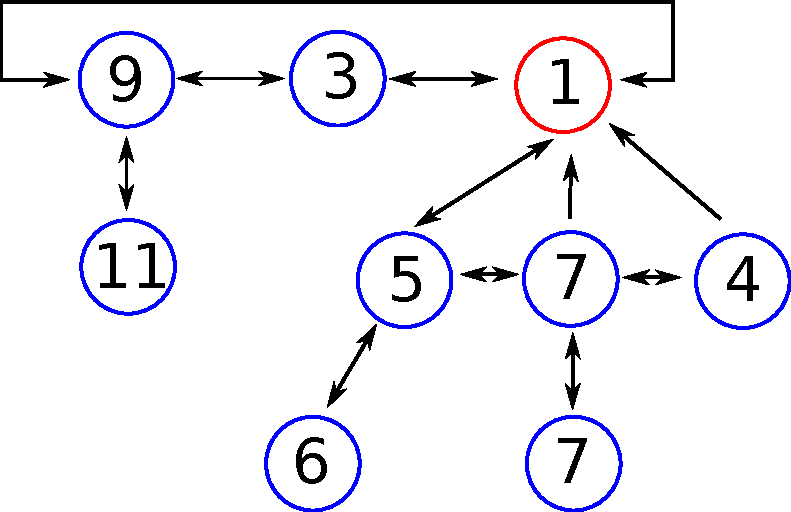
\includegraphics[height=20mm]{images/fibo1.pdf}
	\begin{overprint}
		\onslide<1>
\begin{exampleblock}{Aufbau}
		\begin{itemize}
			\item der Fibonacci-Heap besteht aus gewurzelten B\"aumen
			\item die B\"aume sind \alert{ungeordnet} (anders als im binomial heap)
			\item Gewicht eines Elternknotens $\leq$ Gewicht jedes Kindes
			\item die Liste der Wurzeln ist doppelt verkettet
			\item f\"ur jede Wurzel ist die Liste der Kinder doppelt verkettet
			\item Elemente l\"oschen oder Listen kombinieren in Zeit $O(1)$
		\end{itemize}
	\end{exampleblock}	
	\onslide<2>
\begin{exampleblock}{Aufbau}
		\begin{itemize}
			\item der Heap hat eine Referenz auf das minimale Element
			\item die B\"aume sind nicht notwendigerweise Binomialb\"aume
			\item mit $D(n)$ bezeichnen wir den maximalen Grad eines Fibonacci-Heaps mit Gr\"o\ss e $n$
			\item wir werden zeigen, da\ss\ $D(n)=O(\log n)$
			\item jeder Knoten $v$ hat ferner eine \alert{Markierung} $\mu(v)\in\cbc{0,1}$
		\end{itemize}
	\end{exampleblock}
	\onslide<3>
\begin{exampleblock}{Operationen}
		\begin{description}
			\item[einf\"ugen:] neues Element mit gegebenen Gewicht hinzuf\"ugen
			\item[Minimum:] auffinden des Elements mit minimalen Gewicht
			\item[Minimum entnehmen:] auffinden und entfernen
			\item[Vereinigung:] zwei Heaps zu einem vereinigen
			\item[verringern:] das Gewicht eines Elements verringern
			\item[l\"oschen:] ein Element aus der Datenstruktur entfernen
		\end{description}
	\end{exampleblock}
	\onslide<4>
\begin{exampleblock}{Potentialfunktion}
		\begin{itemize}
			\item $T(\cF)$ bezeichet die Zahl der B\"aume im Fibonacci-Heap $\cF$
			\item $N(\cF)$ bezeichet die Zahl aller Knoten in $\cF$ 
			\item $M(\cF)$ bezeichet die Zahl \alert{markierter Knoten} $v$, d.h.\ $\mu(v)=1$
			\item das \alert{Potential} ist definiert als
				\begin{align*}
					\Phi(\cF)=T(\cF)+2M(\cF)
				\end{align*}
		\end{itemize}
	\end{exampleblock}
	\end{overprint}
\end{frame}

\begin{frame}\frametitle{\mytitle}
	\hfill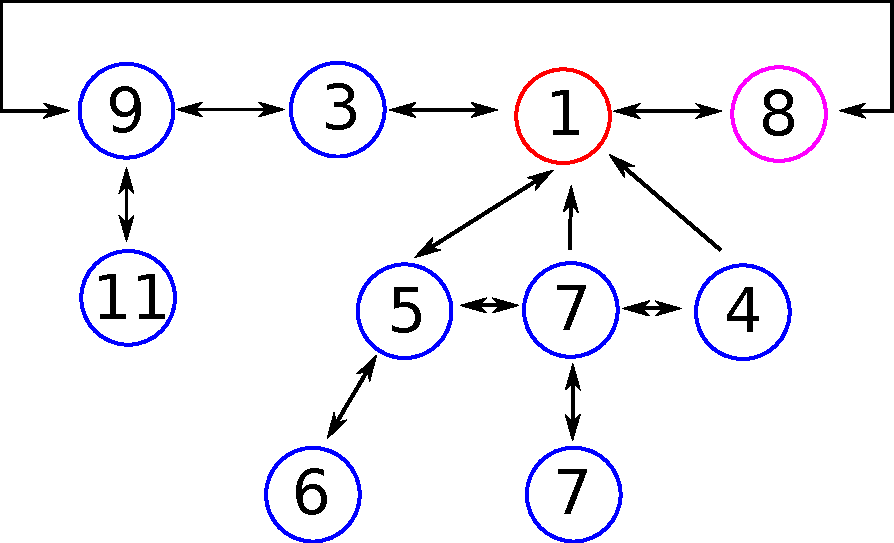
\includegraphics[height=20mm]{images/fibo2.pdf}
	\begin{overprint}
		\onslide<1>
\begin{exampleblock}{Einf\"ugen}
		\begin{itemize}
			\item wir f\"ugen den neuen Eintrag einfach als neuen gewurzelten Baum, bestehend aus einem Knoten, in $\cF$ ein
			\item ggf.\ wird das Minimum aktualisiert
			\item Laufzeit $O(1)$
			\item Potential\"anderung $O(1)$
		\end{itemize}
	\end{exampleblock}	
	\end{overprint}
\end{frame}

\begin{frame}\frametitle{\mytitle}
	\hfill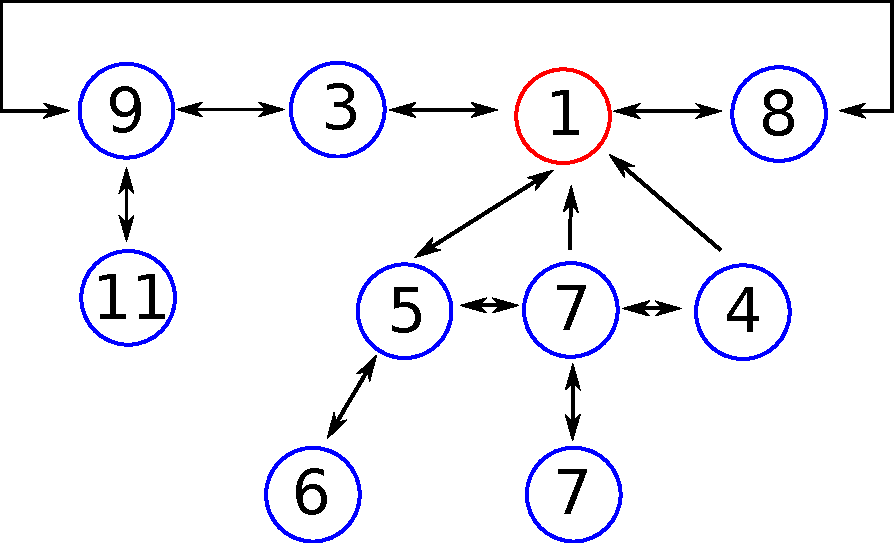
\includegraphics[height=20mm]{images/fibo3.pdf}
	\begin{overprint}
		\onslide<1>
\begin{exampleblock}{Minimum finden}
		\begin{itemize}
			\item der Fibonacci-Heap besitzt eine Referenz auf das minimale Element
			\item Laufzeit $O(1)$; Potential\"anderung $0$
		\end{itemize}
	\end{exampleblock}	
	\end{overprint}
\end{frame}

\begin{frame}\frametitle{\mytitle}
	\begin{overprint}
		\onslide<1>
\begin{exampleblock}{Vereinigung}
		\begin{itemize}
			\item wir f\"ugen einfach die Listen der Wurzeln zusammen
			\item weil sie doppelt verlinkt sind, geht das in Zeit $O(1)$
			\item au\ss erdem wird das Minimum aktualisiert
			\item das Potential \"andert sich nicht
		\end{itemize}
	\end{exampleblock}	
	\end{overprint}
\end{frame}

\begin{frame}\frametitle{\mytitle}
	\begin{overprint}
		\onslide<1-2> 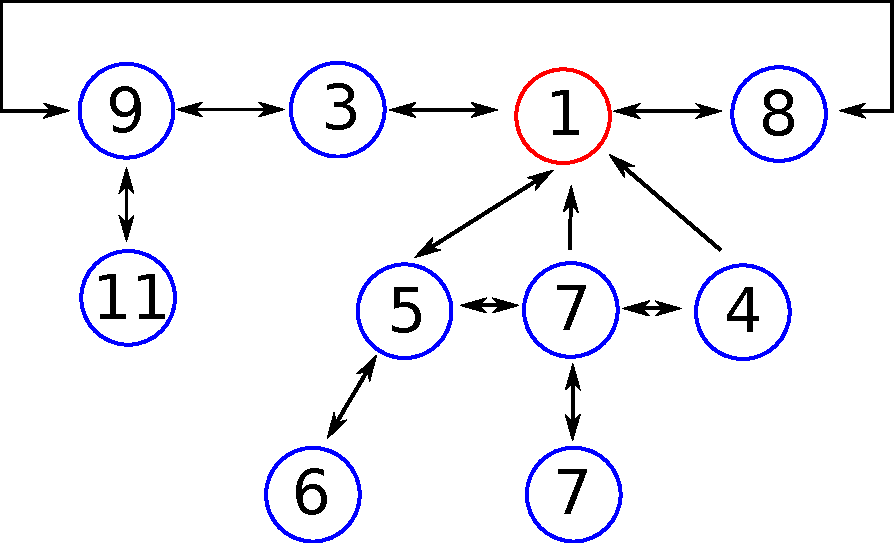
\includegraphics[height=20mm]{images/fibo3.pdf}\hfill 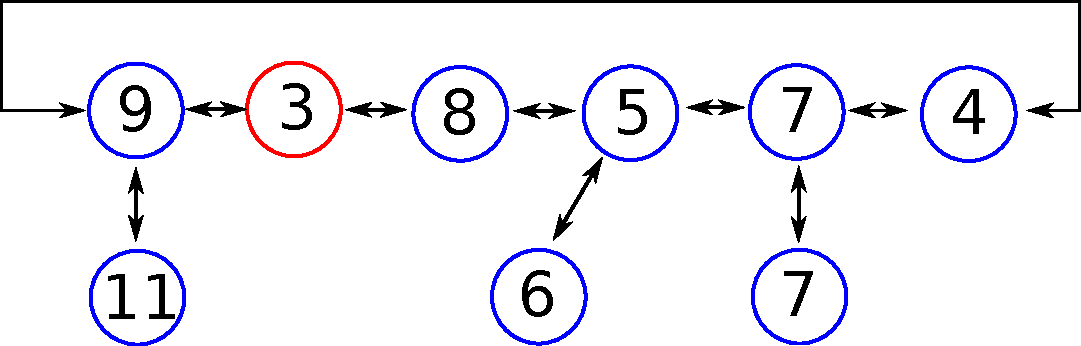
\includegraphics[height=15mm]{images/fibo4.pdf}
		\onslide<3> \hfill 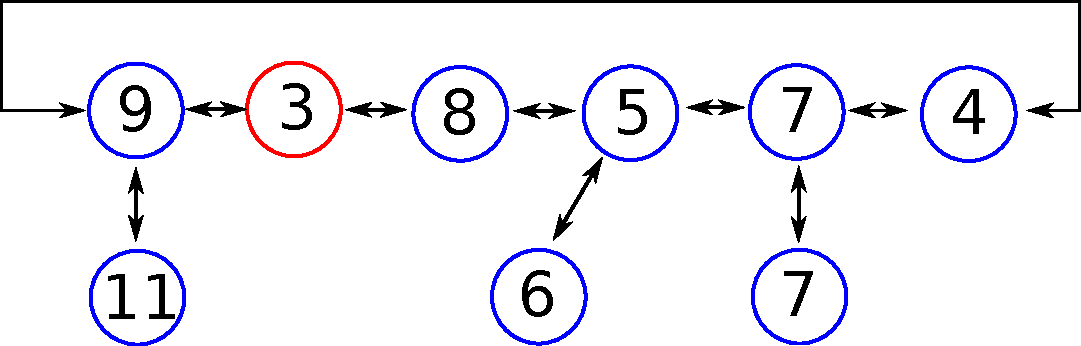
\includegraphics[height=20mm]{images/fibo4.pdf}
		\onslide<4> \hfill 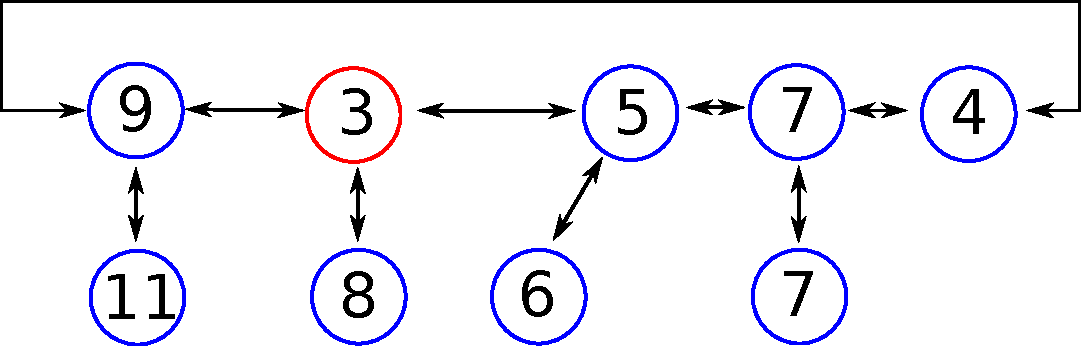
\includegraphics[height=20mm]{images/fibo5.pdf}
		\onslide<5> \hfill 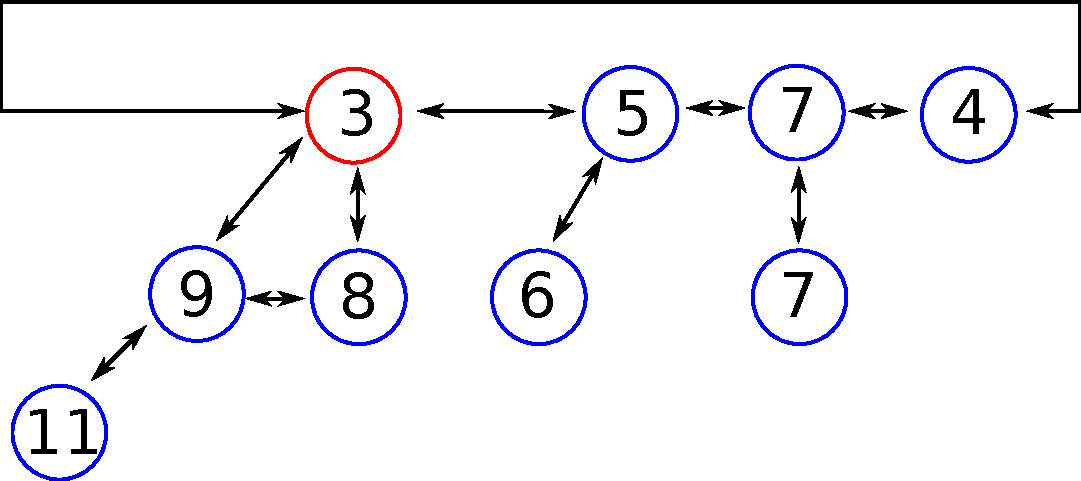
\includegraphics[height=20mm]{images/fibo6.pdf}
		\onslide<6> \hfill 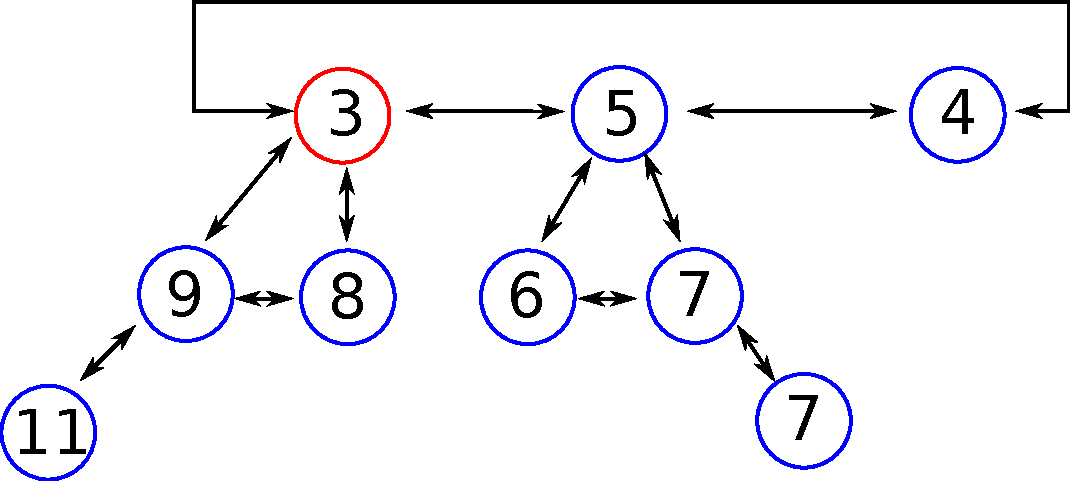
\includegraphics[height=20mm]{images/fibo7.pdf}
		\onslide<7> \hfill 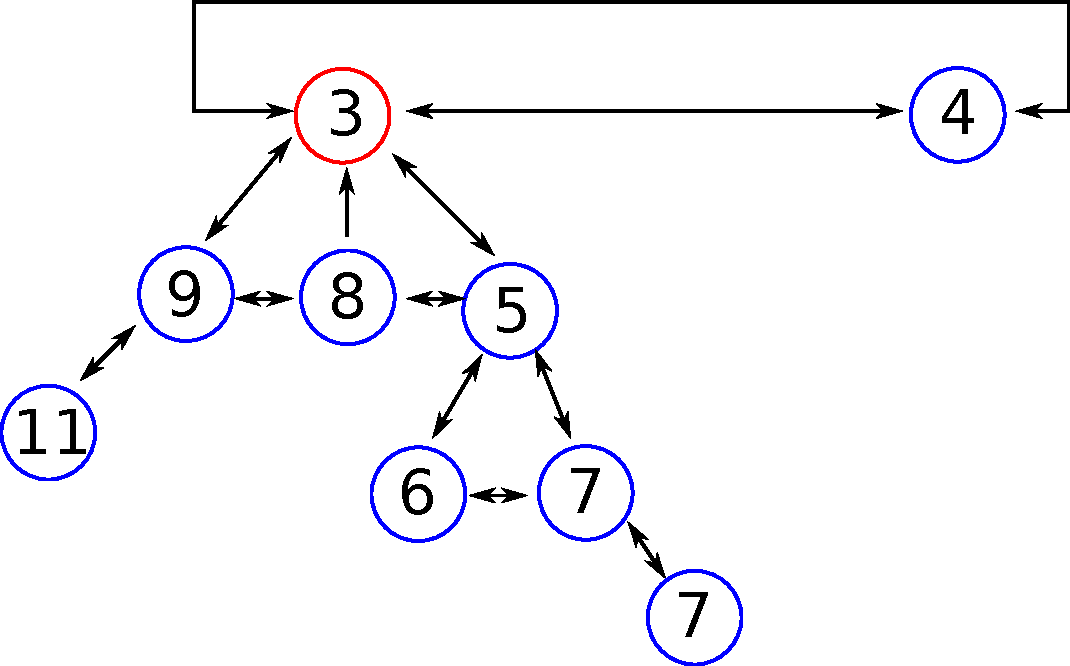
\includegraphics[height=20mm]{images/fibo8.pdf}
	\end{overprint}
	\begin{overprint}
		\onslide<1>
\begin{exampleblock}{Minimum extrahieren}
		\begin{itemize}
			\item das Element minmalen Gewichts wird gel\"oscht
			\item aus jedem Kind des min.\ Elements wird eine neue Wurzel
			\item anschlie\ss end wird der Heap \alert{konsolidiert}
			\item dabei wird auch das Minimum aktualisiert
		\end{itemize}
	\end{exampleblock}	
		\onslide<2>
\begin{exampleblock}{Konsolidieren}
		\begin{itemize}
			\item zum Konsolidieren iterieren wir \"uber die Wurzelliste
			\item wir suchen ein Paar von Wurzeln gleichen Grades
			\item dazu verwenden wir ein Array $A[0\ldots D(N(\cF))]$
			\item $A[i]$ verweist auf eine Wurzel vom Grad $i$ (oder $\emptyset$)
		\end{itemize}
	\end{exampleblock}	
		\onslide<3-7>
\begin{exampleblock}{Konsolidieren}
		\begin{itemize}
			\item wenn zwei Wurzeln gleichen Grades gefunden sind, wird die Wurzel mit gr\"o\ss erem Gewicht wird zum Kind der anderen 
			\item das Feld $\mu(v)$ der Wurzel $v$, die zum Kind der anderen wird, wird auf $0$ gesetzt
			\item der Grad der anderen Wurzel wird um 1 erh\"oht
			\item wir pr\"ufen, ob es eine andere Wurzel dieses neuen Grades schon gibt und wiederholen
		\end{itemize}
	\end{exampleblock}	
	\end{overprint}
\end{frame}

\begin{frame}\frametitle{\mytitle}
\begin{block}{Lemma}
	Die amortisierten Kosten zum Extrahieren des Minimums sind $O(D(N(\cF)))$.
	\end{block}	
\begin{exampleblock}{Beweis}
	\begin{itemize}
		\item sei $\cF'$ der Fibonacci-Heap nach der Extraktion
		\item alle Wurzeln in $\cF'$ haben verschiedene Grade
		\item also $\Phi(\cF')\leq D(N(\cF))+1+2M(\cF)$
		\item folglich $\Phi(\cF')-\Phi(\cF)=O(D(N(\cF)))$
	\end{itemize}
	\end{exampleblock}	
\end{frame}

\begin{frame}\frametitle{\mytitle}
		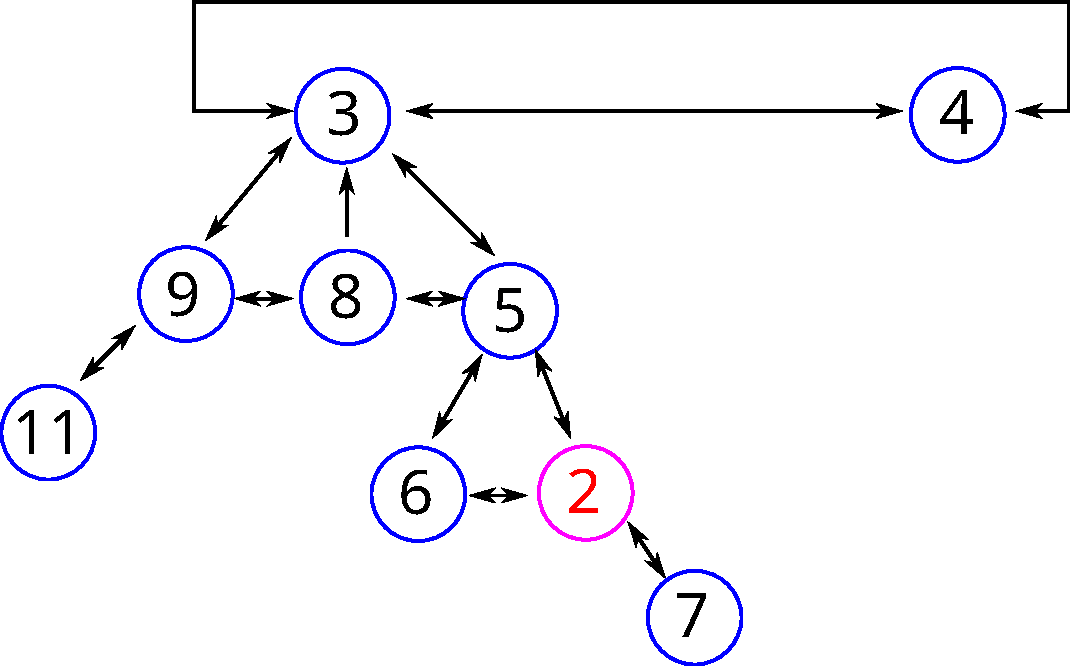
\includegraphics[height=20mm]{images/fibo9.pdf}\hfill 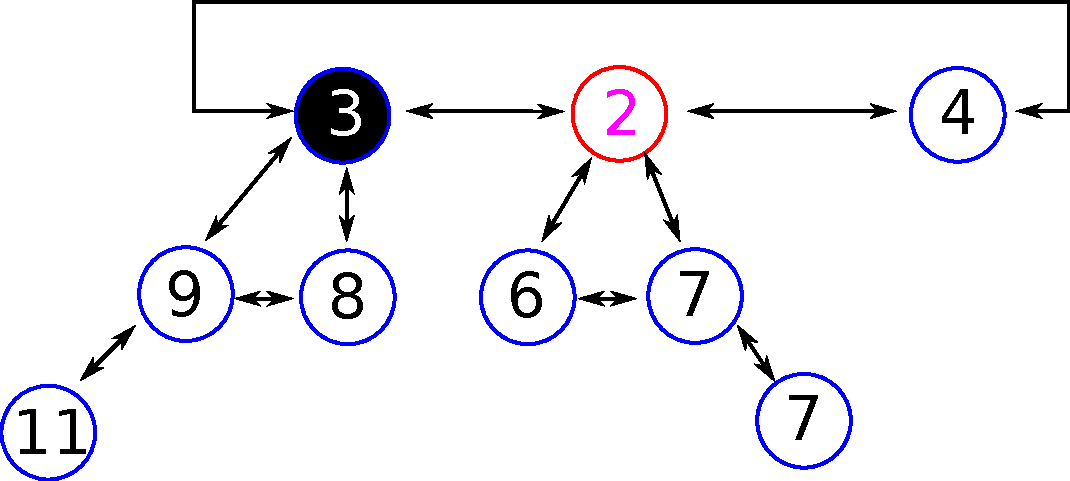
\includegraphics[height=20mm]{images/fibo10.pdf}
	\begin{overprint}
		\onslide<1>
		\begin{exampleblock}{Gewicht verringern}
			\begin{itemize}
				\item wir m\"ussen darauf achten, da\ss\ die Ordnung erhalten bleibt,
				\item d.h.\ Kinder haben mindestens so gro\ss es Gewicht wie Eltern
				\item um den Grad zu begrenzen, trennen wir den Baum ggf.\ auf
				\item dazu verwenden wir die Markierungen
				\item $\mu(x)=1$ zeigt an, da\ss\ $x$ bereits ein Kind verloren hat
			\end{itemize}
		\end{exampleblock}	
		\onslide<2>
		\begin{exampleblock}{Gewicht verringern}
			\begin{itemize}
				\item falls der Knoten $x$, dessen Gewicht reduziert wird, schon eine Wurzel ist, verringern wir einfach das Gewicht, passen ggf.\ das Minimum an und sind fertig
				\item wenn allgemeiner das Gewicht von $x$ nicht kleiner wird als das Gewicht des Elternknotens $y$, gehen wir genauso vor
				\item andernfalls wende die folgende Trennoperation auf $x$ an
			\end{itemize}
		\end{exampleblock}	
		\onslide<3>
		\begin{exampleblock}{Trennen von $x$}
			\begin{itemize}
				\item entferne $x$ aus der Kinderliste von $y$
				\item f\"uge $x$ (und seine Nachkommen) als Wurzel ein
				\item aktualsiere das Minimum
				\item setze $\mu(x)=0$
				\item wende folgende Operation an, um $y$ zu aktualisieren 
			\end{itemize}
		\end{exampleblock}	
		\onslide<4>
		\begin{exampleblock}{Aktualisieren von $y$}
			\begin{itemize}
				\item setze $z$ auf den Elternknoten von $y$
				\item falls $y$ keinen Elternknoten hat, ist nichts zu tun
				\item sonst pr\"ufe, ob $\mu(y)=0$; dann setze $\mu(y)=1$ und stoppe
				\item wenn $\mu(y)=1$, wende Trennen auf $y$ an (und iteriere)
			\end{itemize}
		\end{exampleblock}	
		\onslide<5>
		\begin{exampleblock}{Amortisierte Laufzeit}
			\begin{itemize}
				\item sei $\cF'$ der Heap nach der Extraktion
				\item ein neuer Baum, der in die Wurzelliste eingef\"ugt wird, stammt von einem Knoten $u$, dessen Markierung $\mu(u)$ die Trennoperation von $1$ auf $0$ setzt
				\item einzige Ausnahme ist ggf.\ der extrahierte Knoten
			\end{itemize}
		\end{exampleblock}	
		\onslide<6>
		\begin{exampleblock}{Amortisierte Laufzeit}
			\begin{itemize}
				\item wenn $t$ neue B\"aume in die Wurzelliste eingef\"ugt werden, \"andert sich das Potential also um
					$$\Phi(\cF')-\Phi(\cF)\leq t-2t+1\leq 1-t$$
				\item dem steht eine materielle Laufzeit von $O(t)$ gegen\"uber
				\item die amortisierte Laufzeit ist also $O(1)$
			\end{itemize}
		\end{exampleblock}	
	\end{overprint}
\end{frame}

\begin{frame}\frametitle{\mytitle}
	\begin{overprint}
		\onslide<1>
		\begin{exampleblock}{Entfernen eines Knotens}
			\begin{itemize}
				\item verringere das Gewicht des zu entfernenden Knotens auf $-\infty$
				\item extrahiere anschlie\ss end den Knoten geringsten Gewichts
				\item amortisierte Laufzeit ist $O(D(N(\cF)))$
			\end{itemize}
		\end{exampleblock}	
	\end{overprint}
\end{frame}

\begin{frame}\frametitle{\mytitle}
	\begin{overprint}
		\onslide<1>
		\begin{block}{Proposition}
			Der maximale Grad eines Fibonacci-Heap $\cF$ ist $O(\log N(\cF))$.
		\end{block}	
		\onslide<7>
		\begin{exampleblock}{Amortisierte Laufzeiten}
			Aus der Proposition und unserer obigen Analyse ergeben sich die folgenden amortisierten Laufzeiten f\"ur den Fibonacci-Heap:
			\begin{description}
				\item[einf\"ugen:] $O(1)$
				\item[Minimum:] $O(1)$
				\item[Minimum entnehmen:] $O(\log n)$
				\item[Vereinigung:] $O(1)$
				\item[verringern:] $O(1)$
				\item[l\"oschen:] $O(\log n)$
			\end{description}
		\end{exampleblock}
		\onslide<2>
		\begin{block}{Lemma}
			Angenommen Knoten $x$ des Fibonacci-Heaps $\cF$ hat $k$ Kinder $y_1,\ldots,y_k$, numeriert nach der Reihenfolge, in der sie an $x$ angef\"ugt worden sind.
			Dann gilt hat $y_i$ mindestens $i-2$ Kinder ($i=2,\ldots,k$).
		\end{block}	
		\begin{exampleblock}{Beweis}
			\begin{itemize}
				\item zu dem Zeitpunkt, als $y_i$ an $x$ angef\"ugt wurde, hatte $x$ bereits mindestens $i-1$ Kinder
				\item ein Knoten wird nur dann als Kind an einen anderen angeh\"angt, wenn beide den gleichen Grad haben
				\item seitdem $y_i$ an $x$ angeh\"angt wurde, hat $y_i$ h\"ochstens ein Kind verloren (weil im Fall $\mu(y)=1$ der Knoten $y$ selbst zur Wurzel wird, wenn er noch ein Kind verliert)
			\end{itemize}
		\end{exampleblock}
		\onslide<3>
		\begin{exampleblock}{Erinnerung: die Fibonacci-Zahlen}
			\begin{itemize}
				\item $F_0=0$
				\item $F_1=1$
				\item $F_k=F_{k-1}+F_{k-2}$ f\"ur $k\geq2$
				\item also erhalten wir f\"ur $\ell\geq0$,
					\begin{align*}
						F_{\ell+2}&=1+\sum_{i=0}^\ell F_i\geq\bcfr{1+\sqrt 5}2^\ell
					\end{align*}
			\end{itemize}
		\end{exampleblock}
		\onslide<4>
		\begin{block}{Lemma}
			F\"ur einen Knoten $x$ in einem Fibonacci-Heap $\cF$ sei $N(x,\cF)$ die Zahl der Nachkommen von $x$, einschlie\ss lich $x$ selbst. Wenn $\ell$ die Zahl der Kinder von $x$ ist, gilt $ N(x,\cF)\geq F_{\ell+2} $.
		\end{block}
		\begin{exampleblock}{Beweis}
			\begin{itemize}
				\item Induktion nach $\ell$
				\item sei $s_\ell$ die kleinstm\"ogliche Zahl von Nachkommen eines Knotens mit $\ell$ Kindern
				\item wir sehen unmittelbar, da\ss\ $s_0=1$ und $s_1=2$
				\item seien nun allgemeien $y_1,\ldots,y_k$ die Kinder von $x$ in $\cF$
				\item Knoten $y_i$ habe $\ell_i$ Kinder
				\item dann gilt $\ell_i\geq i-2$
			\end{itemize}
		\end{exampleblock}
		\onslide<5>
		\begin{exampleblock}{Beweis (fortgesetzt)}
			\begin{itemize}
				\item ferner gilt $s_{h+1}\geq s_h$
				\item also erhalten wir mit Induktion und dem vorherigen Lemma
					\begin{align*}
						s_\ell&\geq2+\sum_{i=2}^\ell s_{\ell_i}\geq2+\sum_{i=2}^\ell s_{i-2}\\
							  &\geq2+\sum_{i=2}^\ell F_{i}>F_{\ell+2}
					\end{align*}
				\item weil $N(x,\cF)\geq s_\ell$, folgt die Behauptung
			\end{itemize}
		\end{exampleblock}
		\onslide<6>
		\begin{exampleblock}{Beweis der Proposition}
			\begin{itemize}
				\item das Lemma zeigt, da\ss\ f\"ur jeden Knoten $x$ mit $\ell$ Kindern gilt
					\begin{align*}
						N(x,\cF)\geq F_{\ell+2}\geq\bcfr{1+\sqrt 5}2^\ell
					\end{align*}
				\item also folgt $D(\cF)\leq O(\log N(\cF))$
			\end{itemize}
		\end{exampleblock}
	\end{overprint}
\end{frame}

\begin{frame}\frametitle{\mytitle}
	\begin{overprint}
		\onslide<1>
		\begin{exampleblock}{Zusammenfassung}
			\begin{itemize}
				\item Fibonacciheaps sind die effizienteste Datenstruktur f\"ur den Dijkstra-Algorithmus
				\item die Laufzeit von Dijkstra mit Fibonacciheaps betr\"agt
					\begin{align*}
						O(|E|+|V|\log|V|)
					\end{align*}
				\item Die Laufzeit wir mit Hilfe der \alert{amortisierten Analyse} abgesch\"atzt
			\end{itemize}
		\end{exampleblock}
	\end{overprint}
\end{frame}

\end{document}
